\documentclass[]{article}
\usepackage{fullpage}
\usepackage{listings}
\usepackage{graphicx}
\usepackage{epstopdf}
\usepackage{bbding}
\usepackage{float}
\usepackage[paperwidth=8.5in, paperheight=11in]{geometry}

\newcommand*\good{\item[\Checkmark]}
\newcommand*\bad{\item[\XSolidBrush]}

\lstset{numbers=left}

%opening

\title{Project Beta Report\\\textit{Squirrel Quarrel: Protect Your Nuts Edition}}
\author{Matt Coley\\David Ickert\\}


\begin{document}
	\maketitle
	\newpage
	\tableofcontents
	\newpage
	\section{Summary of Milestones}
	\subsection{Work Performed \& Required Breakdown}
		Even before beginning on the project, it became clear that many of our original labor divisions overlapped.  For example, the original plan was for Matt to implement the map and for David to implement the movement and resctritions of that.  However, this became a simple process for Matt to complete as part of the Map class development.  We will attempt to maintain the division between tasks as originally planned, but as the project proceeds, it is easier to complete tasks on an ``as needed and what is next'' basis.
		
		Below is a list of the original milestones.  Checkmarks represent a completed tasks, while an ``X'' is an incomplete task.  Additional new information is provided in bold.
		\subsubsection{First Milestone: Project Organization}
		Estimated Time: Half a day to one day.\\
		\textbf{Actual Time Used: About an hour.}\\
		Assigned To: David Ickert
		\begin{enumerate}
			\good Create project. \textbf{(David Ickert)}
			\good Create empty files and folders based on the estimated UML diagrams. \textbf{(David Ickert)}
			\good Implement class inheritance. \textbf{(David Ickert)}
			\good Setup version control (such as GitHub). \textbf{(David Ickert)}
		\end{enumerate}		
		\subsubsection{Second Milestone: Initial Implementation \& Map}
		Estimated Time: 3 days to one week.\\
		\textbf{Actual Time Used: ???}\\		
		Assigned To: Matt Coley 
		\begin{enumerate}
			\good Display the map. \textbf{(Matt Coley)}
			\good Pan the map. \textbf{(Matt Coley)}
			\bad Place the home tree in the center of the map.
			\bad Randomly place obstacles.
			\bad Randomly place nuts (check for collision with obstacles).
			\bad Randomly place enemies (check for collisions with obstacles and nuts).
		\end{enumerate}	
		\subsubsection{Third Milestone: Sprites, Animations, and Basic Controls}		
		Estimated Time: 3 days to one week.\\
		\textbf{Actual Time Used So Far: About 2-3 Hours.}\\
		Assigned To: David Ickert
		\begin{enumerate}
			\bad Replace the placeholders with sprites.
			\good Implement character animations. \textbf{(David Ickert)}
			\good Implement basic movement controls. \textbf{(Matt Coley as part of the map class)}
			\good Ensure restricted movement. \textbf{(Matt Coley as part of the map class)}
		\end{enumerate}			
		\subsubsection{Fourth Milestone: Implement Menus \& Refine Controls}
		Estimated Time: 3 to 5 days.\\
		Assigned To: Matt Coley 	
		\begin{enumerate}
			\bad Create main menu \& pause menu.
			\bad Implement the functionality of the menus.
			\bad Refine the controls.
		\end{enumerate}			
		\subsubsection{Fifth Milestone: Player Logic: Actions \& Combat}
		Estimated Time: One to two weeks.\\
		Assigned To: David Ickert
		\begin{enumerate}
			\bad Implement the scoring system.
			\bad Implement the powering up logic.
			\bad Create collision detection for projectiles.
			\bad Bust-a-nut special move.
		\end{enumerate}			
		\subsubsection{Sixth Milestone: A* Path Finding}
		Estimated Time: To the end of project.\\
		Assigned To: Matt Coley and David Ickert
		\begin{enumerate}
			\bad Initial A* path finding implementation.
		\end{enumerate}			
		\subsubsection{Seventh Milestone: Enemy AI \& Combat}
		Estimated Time: One to two weeks.\\
		Assigned To: Matt Coley
		\begin{enumerate}
			\bad Enemies navigate towards player.
			\bad Attack the player.
			\bad Refine A* as needed.
		\end{enumerate}		
		\subsubsection{Eighth Milestone: Implement User Interface}
		Estimated Time: 3 days to one week.\\
		Assigned To: David Ickert
		\begin{enumerate}
			\bad Create UI graphics.
			\bad Manage logic behind UI.
			\bad Proper positioning and display of UI elements.
			\bad Statistics screen.
		\end{enumerate}		
		\subsubsection{Ninth Milestone: Polish \& Code Refinement}
			Estimated Time: As time permits.\\
			Assigned To: Matt Coley and David Ickert		
	\section{Challenges}
		\subsection{Getting Started}
			One of the first challenges we faced was getting started.  Consequently, we met an additional time to discuss how we should proceed and to examine some questions that arose since the project proposal.  One topic of discussion was how to handle the map.  We decided, based on its uniqueness, to create it as its own class with its own draw and update methods.  We also discussed the size of the map and concluded that 2400 x 1800 pixels are sufficient.  However, this is arbitrary and subject to change.  Based on the types of objects in the game, we decided on the best draw order, game compents order, and discussed several possible game states.\\\\
			\textbf{Draw Order (back to front)}
			\begin{enumerate}
				\item Map
				\item Powerups
				\item Nuts
				\item Player
				\item Enemies
				\item Obstacles
				\item Hometree
				\item Menu
			\end{enumerate}
			\textbf{Game Component Order}
			\begin{enumerate}
				\item Map
				\item SpriteManager
				\item Menu
			\end{enumerate}
			\textbf{Possible Game States}
			\begin{enumerate}
				\item Active - When the game is being played.
				\item Paused - A menu is displayed in the game.
				\item Main\_Menu
				\item Game\_Over
				\item New\_Round - Generate a new map.
			\end{enumerate}
		\subsection{The Sprite Class (David Ickert)}
			We quickly realized that the game engine did not need the original planned base class, GameObject.  This class, from which all other classes derived from, had one attribute for position and two methods for the size.  Since our game is 2D, and everything is composed of sprites, we decided to change the base class to an abstract Sprite class.  This has the same capabilities as the GameObject, but adds textures, and extends to cover most other classes from static sprites to animated characters.  More important, we incorporation two new virtual methods that allow polymorphism for update and draw.  Each sprite in the game now updates and draws itself.  This removes large amounts of code from the base update and adds a new layer of abstraction.
			\begin{figure}[H]
				\centering
				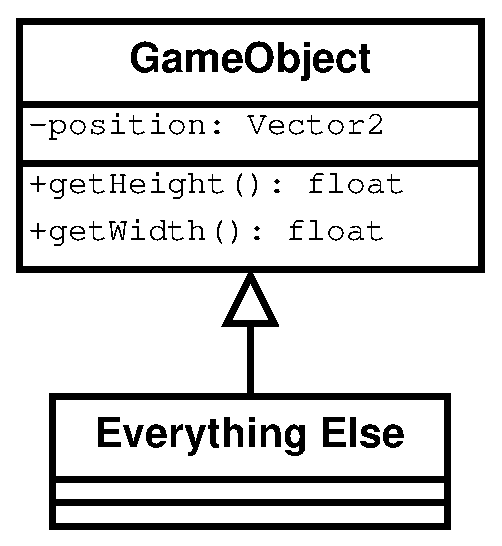
\includegraphics[scale=0.50]{UML/GameObject}
				\caption{Abandoned Original GameObject Class}				
			\end{figure}
			\begin{figure}[H]
				\centering
				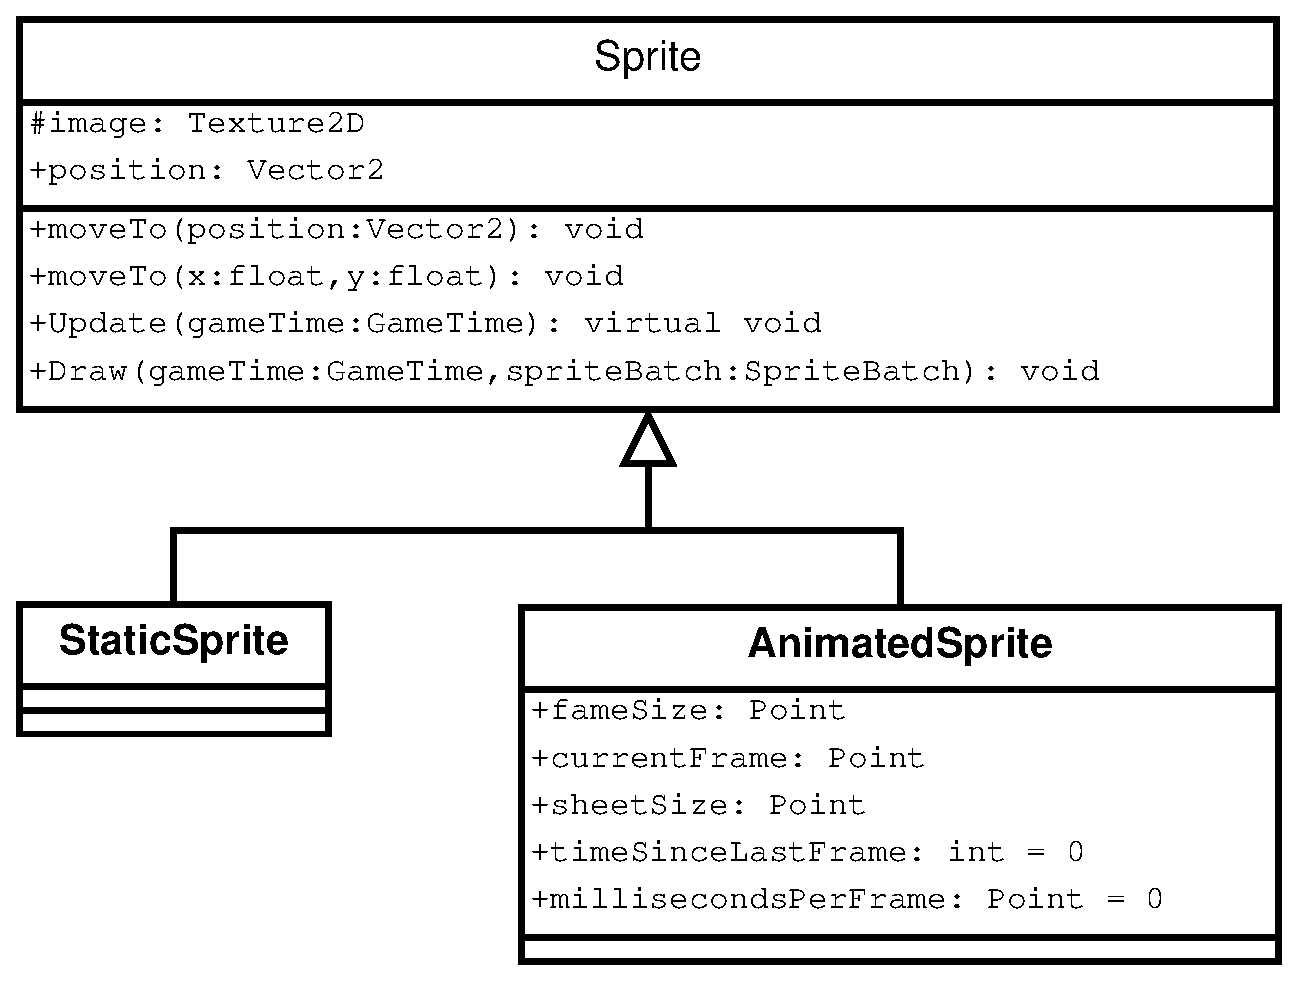
\includegraphics[scale=0.50]{UML/Sprite}
				\caption{New Sprite Class}				
			\end{figure}
			
			Creating the AnimatedSprite class was not too difficult.  The most challenging aspect is the how to make changes during the update method to show the correct sequence.  The first few attempts either did not animation correct or animated is distrubing ways.  I expect that this class will need to be extended to handle multiple animations per a sprite sheet.  For example,  a character needs two unique animations when walking north versus walking south.  For now, I used a simple sprite sheet I found online for testing.
			
			\begin{figure}[H]
				\centering
				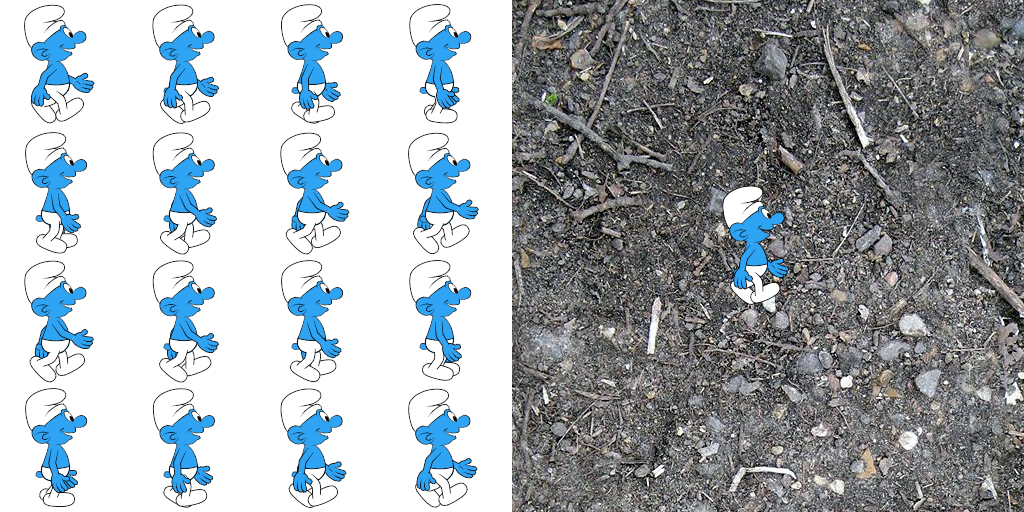
\includegraphics[scale=0.40]{UML/SpriteSampleScreen}
				\caption{Left: Sample Sprite Sheet, Right: Animated on Matt's Map}
			\end{figure}
			
		\subsection{The SpriteManager (David Ickert)}
			Our changes from the GameObject base class to the Sprite base class lead to the development of the SpriteManager class.  This is the first XNA game component of the project and it has several important functions in the game engine.  First, it overrides both the update and draw method to call each sprites respective methods.  Second, it ensures that the game draws each sprite in the correct order previously discussed.  Finally, it adds that additional layer of abstraction and removes more code from the base update and draw methods.
		\subsection{The Map (Matt Coley)}
			When getting ready to implement the map, we realized that the map will end up being quite large, when measured in pixels.  This meant our initial idea of creating a solid background texture would have been too large and hindered performance too much.  We solved this problem by creating a tiled background texture that can repeat a ground pattern which is restricted to our texture size limits.  The map also needed the ability to pan.  This proved a larger task than we initially anticipated.  We did not want to over-complicate the logic by introducing a camera, so we decided to make the map pan and leave the player in the same spot relative to the screen boundaries.  This also meant that every item on the map needed to be updated whenever the player moved.  We decided that the time saved and complications avoided with camera movement where worth the performance hit of the extra position updates each frame.
		\subsection{Game Menu (Matt Coley)}
			The game menu was fairly simple to set up.  We decided to keep the menu drawing separate from the sprite manager.  This allowed us to work simultaneously on both parts.  Also, the rendering requirements for the menu system were very slim.  We have basic pause, continue, and quit game functionality in the game menu.
		\subsection{Main Menu (Matt Coley)}
			
			
\end{document}
